\documentclass{article}
\usepackage[margin=1in]{geometry}
\usepackage{tikz, amsmath, amssymb, fancyhdr, xfrac, physics}

\usetikzlibrary{patterns}

% \pagecolor[rgb]{0.2,0.2,0.2}
% \color[rgb]{1,1,1}

\pgfdeclarepatternformonly{south west lines}{\pgfqpoint{-0pt}{-0pt}}{\pgfqpoint{3pt}{3pt}}{\pgfqpoint{3pt}{3pt}}{
        \pgfsetlinewidth{0.05pt}
        \pgfpathmoveto{\pgfqpoint{0pt}{0pt}}
        \pgfpathlineto{\pgfqpoint{3pt}{3pt}}
        \pgfpathmoveto{\pgfqpoint{2.8pt}{-.2pt}}
        \pgfpathlineto{\pgfqpoint{3.2pt}{.2pt}}
        \pgfpathmoveto{\pgfqpoint{-.2pt}{2.8pt}}
        \pgfpathlineto{\pgfqpoint{.2pt}{3.2pt}}
        \pgfusepath{stroke}}

% Headers
\pagestyle{fancy}
\fancyhf{}
\rhead{Max Ortner}
\lhead{Complex Variables}
\chead{Problem Set I}
\cfoot{Page \thepage}
\renewcommand{\headrulewidth}{0pt}
\renewcommand{\footrulewidth}{0pt}

\newcommand{\nhat}[1]{\boldsymbol{\hat{\textbf{#1}}}}

\newcommand{\qnumber}[1]{
\vspace{0.5cm}
\noindent
\textbf{#1.}
\vspace{4mm}
}

\setlength{\parskip}{0.15cm}
\setlength{\parindent}{0em}
\renewcommand{\baselinestretch}{1.2}

\begin{document}

\begin{center}
    \huge Complex Variables
    
    \large Problem Set I
    \thispagestyle{plain}
\end{center}

\qnumber{1}

To find the multiplicative inverse of a complex number, $z=2-5i$, we must identify another complex number $z^{-1}$ that satisfies the property that when multiplied with $z$, the real number 1 is yielded. We can consider each number to be an ordered pair where $z^{-1}=(u, v),$ and $u,v\in\mathbb{R}$. Therefore, $z^{-1}$ must be such that
\[
    (2,-5)(u,v)=(1,0).  
\]
Distributing each term and combining yields the equation
\[
    (2u+5v, 2v-5u)=(1,0),
\]
which can be written as the series of equations
\[
\begin{split}
    2u+5v&=1, \\
    2v-5u&=0.
\end{split}
\]
We can find the value of $u$ through the use of the first equation to get
\[
    u=\frac{-5v+1}{2}.  
\]
You can substitute this value into the second equation to get a quantitative definition of $v$,
\[
    v=\frac{5}{29}.  
\]
Substituting this back into the equation to solve for $u$ yields the value of $z^{-1}$ to be
\[
    z^{-1}=\frac{2}{29}+\frac{5}{29}i.  
\]

\qnumber{2}

The quotient of two complex numbers, $z_1, z_2\in\mathbb{C}$,  can be expressed as multiplication of one and the other in terms of its multiplicative inverse, or
\[
    \frac{z_1}{z_2}=z_1 z_2^{-1}.
\]
For the quotient in question, $z_1=1+2i$ and $z_2=2-3i$. Therefore, in order to expand the previous equation, we must find the multiplicative inverse of $z_2$, which can be found using the methods of the previous answer to be
\[
    z_2^{-1}=\frac{2}{13}+\frac{3}{13}i.  
\]
Now, expanding the quotient and simplifying, we get
\[
    z_1 z_2^{-1}=-\frac{4}{13} + \frac{7}{13}i.
\]

\qnumber{3}

\begin{figure}[h]
    \centering

    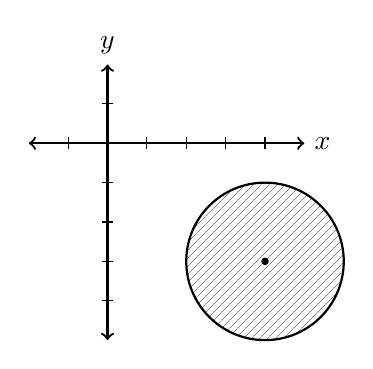
\begin{tikzpicture}[scale=0.5]
        \draw[<->, thick] (-2,  0) -- (5, 0) node[right] {$x$};
        \draw[<->, thick] ( 0, -5) -- (0, 2) node[above] {$y$};

        % X-Axis lines
        \foreach \i in { -1, 0, ..., 3, 4 } 
        {
            \draw[thin] (\i, -0.15) -- (\i, 0.15);
        }

        % Y-Axis lines
        \foreach \i in { -4, -3, ..., 0, 1 } 
        {
            \draw[thin] (-0.15, \i) -- (0.15, \i);
        }

        \draw[thick, pattern color=black, pattern=south west lines] (4, -3) circle(2);
        \draw[fill]  (4, -3) circle(0.08);

    \end{tikzpicture}

    \caption{A circle centered at (4, -3) with a radius of 2.}
\end{figure}

Let there exist a complex number $z=x+iy$ where $x, y \in \mathbb{R}$. With the given the inequality $|3z-12+9i|\leq 6$, we can substitute in our definition of $z$ and simplify to get
\[
    |(x-4) + (y+3)i|\leq 2.
\]
This is the equation for the area inside of a circle with its origin at $(4, -3)$ and its radius $r=2$. A graphical representation is shown above.

\qnumber{4}

\begin{figure}[h]
    \centering

    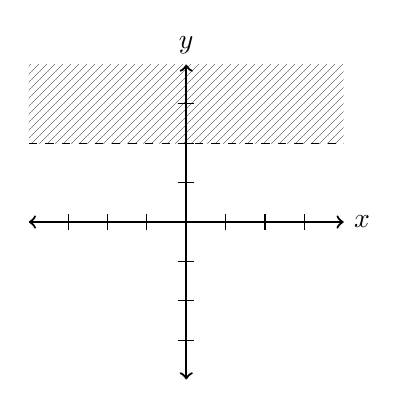
\begin{tikzpicture}[scale=2]
        
        \draw[<->, thick] (-1,  0) -- (1, 0) node[right] {$x$};
        \draw[<->, thick] ( 0, -1) -- (0, 1) node[above] {$y$};

        % X-Axis lines
        \foreach \i in { -0.75, -0.5, ..., 0.5, 0.75 } 
        {
            \draw[thin] (\i, -0.05) -- (\i, 0.05);
        }

        % Y-Axis lines
        \foreach \i in { -0.75, -0.5, ..., 0.5, 0.75 } 
        {
            \draw[thin] (-0.05, \i) -- (0.05, \i);
        }

        \draw[thin, pattern color=black, pattern=south west lines, draw=none] (-1, 0.5) rectangle (1, 1);

        \draw[dashed] (-1, 0.5) -- (1, 0.5);

    \end{tikzpicture}
    
\end{figure}

In order to consider the set of complex numbers that satisfy the inequality $\text{Re}(iz+2)>0$, consider the complex number $z=x+iy$, where $x,y\in\mathbb{R}$. We can substitute and simplify the inside of the real expression to get
\[
    iz+2=-(y-2)+xi,
\]
whose real component is $-(y-2)$. Therefore, the inequality is
\[
    -(y-2)>0,
\] 
or $y>2$. The graphical representation of this is shown above.

\newpage

\qnumber{5}

To find the angle of the complex number $z=-6+6i\sqrt{3}$, we can find the complex number $\hat{z} \in \mathbb{C}$ such that $|\hat{z}|=1$ and the real components of $\hat{z}$ and $z$ are proportional by a scalar $c\in\mathbb{R}$, or
\[
\begin{split}
    \hat{z}&=c(6i\sqrt{3}-6), \\
    1&=c|z|.
\end{split}
\]
The second equation relates the magnitude of $\hat{z}$ and $z$. Solving for $\hat{z}$ yields
\[
    \hat{z}=-\frac{1}{2}+i\frac{\sqrt{3}}{2}.
\]  
To find the angle of this number relative to the real line, consider the identity 
\[
    \arccos (-\frac{1}{2})=\frac{2\pi}{3}.    
\]
We can now express $\hat{z}$ in terms of its angle with the real axis with
\[
    \hat{z}=\cos (\frac{2\pi}{3}) + i\sin (\frac{2\pi}{3}).
\]
To transform $\hat{z}$ into $z$, we must multiply it by $\frac{1}{c}$ or $|z|=12$, so
\[
    z=12\cos (\frac{2\pi}{3}) + 12i\sin (\frac{2\pi}{3}).
\]

\qnumber{6}

To put a complex number $z^n, z\in\mathbb{C}, n\in\mathbb{R}$ into exponential form, consider first the exponential form of $z$ by itself. In the given case, $z=1+i$. It is obvious that its magnitude is $\sqrt{2}$ and the angle is $\frac{\pi}{4}$ with the positive real axis. Therefore, its exponential form is
\[
    1+i=\sqrt{2}e^{ i\frac{\pi}{4} }.  
\]
If $n=8$, we can raise both sides of the equation to get our equivalency to $z^8$:
\[
    (1+i)^8=16 e^{ 2\pi i }=16.
\]

\qnumber{7}

To find the principal argument of a complex number $z=-2+2i$, we need to know the angle it makes with the real axis. Since both components are the same magnitude we can easily conclude it makes a $\frac{\pi}{4}$ radian triangle directed in the second quadrant. Therefore the angle is $\frac{\pi}{4}+\frac{\pi}{2}=\frac{3\pi}{4}$. Since this angle lies within the range $-\pi<\theta\leq\pi$, 
\[
    \text{Arg } z = \frac{3\pi}{4},  
\]
and its general argument is
\[
    \arg z = \frac{3\pi}{4} + 2\pi n,\;\;n\in\mathbb{Z}.  
\]

\qnumber{8}

\begin{figure}[h]
    \centering
    
    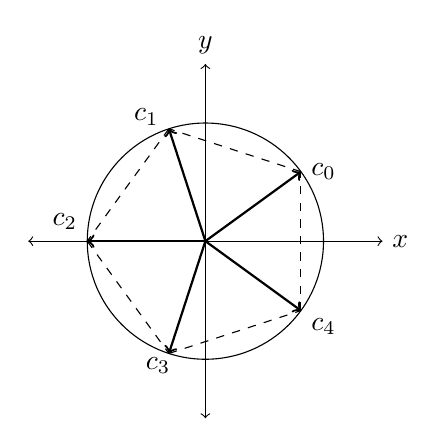
\begin{tikzpicture}[scale=1.5]
    
    \draw [<->] (-1.5, 0) -- (1.5, 0) node[right] {$x$};
    \draw [<->] (0, -1.5) -- (0, 1.5) node[above] {$y$};
    
    \draw[->, thick] (0, 0) -- ( 0.809, 0.588) node[above, right] {$c_0$};
    \draw[->, thick] (0, 0) -- (-0.309, 0.951) node[above=0.15cm, left] {$c_1$};
    \draw[->, thick] (0, 0) -- (-1, 0) node[above=0.25cm, left] {$c_2$};
    \draw[->, thick] (0, 0) -- (-0.309, -0.951) node[below=0.15cm, left=-0.15cm] {$c_3$};
    \draw[->, thick] (0, 0) -- ( 0.809, -0.588) node[below=0.2cm, right] {$c_4$};
    
    \draw[dashed, thin] ( 0.809, 0.588) -- (-0.309, 0.951);
    \draw[dashed, thin] (-0.309, 0.951) -- (-1, 0);
    \draw[dashed, thin] (-1, 0) -- (-0.309, -0.951);
    \draw[dashed, thin] (-0.309, -0.951) -- ( 0.809, -0.588);
    \draw[dashed, thin] ( 0.809, -0.588) -- ( 0.809, 0.588);
    
    \draw (0, 0) circle  (1);
    
    \end{tikzpicture}
    
\end{figure}

Although $-7$ is a real number, it can be expressed as the complex number $-7+0i$. Therefore, we can describe it in exponential form as
\[
    -7=7e^{i(\pi + 2\pi n)},\;\;n\in\mathbb{Z}.
\]
Note, the $n$ accounts for the fact that you can add any number of $2\pi$'s and end up in the same spot. To find the fifth root of $-7$, we can simply take the fifth root of either side to obtain
\[
    \sqrt[5]{-7}=\sqrt[5]{7}e^{ i(\frac{\pi}{5}+\frac{2\pi n}{5}) }.  
\]
To find the distinct roots, we should find the complex values where $n\leq 5$. Therefore, let $c_n$ be the complex root at $n$. Each distinct root $n$ is
\[
\begin{split}
    c_1&=\sqrt[5]{7} e^{ i(\frac{\pi}{5}) }, \\
    c_2&=\sqrt[5]{7} e^{ i(\frac{\pi}{5} + \frac{2\pi}{5}) }, \\
    c_3&=\sqrt[5]{7} e^{ i(\frac{\pi}{5} + \frac{4\pi}{5}) }, \\
    c_4&=\sqrt[5]{7} e^{ i(\frac{\pi}{5} + \frac{6\pi}{5}) }, \\
    c_5&=\sqrt[5]{7} e^{ i(\frac{\pi}{5} + \frac{8\pi}{5}) }.
\end{split}
\]
Each point $c_n$ is shown graphically in the illustration above.

\qnumber{9}

Consider the complex polynomial $z^2+4z+5$ where $z\in\mathbb{C}$. Let $z=x+yi,\;x,y\in\mathbb{R}$. We can thus write the polynomial as
\[
    (x+yi)^2+4(x+yi)+5=0.  
\]
Let's consider each term to be an ordered pair, $z=(x,y)$. We can write this as
\[
    (x^2-y^2, 2xy) + (4x, 4y) + (5, 0) = (0, 0).
\]
In this notation, it becomes clear there exists a system of two equations, namely
\[
\begin{split}
    x^2-y^2+4x+5&=0, \\
    2xy + 4y &= 0.
\end{split}
\]
The second equation can be solved for both $x$ and $y$ yielding $x=-2$ and $y=0$ as solutions. Now to find their corresponding component pair, we simply plug one value and solve for the other in the first equation. For a choice of $x=-2$, $y=\pm 1$, and for a choice of $y=0$, $x=1$ and $x=-5$. Therefore we have the solutions $z_n\in\mathbb{C}$,
\[
\begin{split}
    z_1 &= -2 + i, \\
    z_2 &= -2 - i, \\
    z_3 &=  1, \\ 
    z_4 &= -5.
\end{split}
\]

\qnumber{10}

Let there be an integer $n>0$. In order for $i$ to be a root of 1,
\begin{equation} \label{eq:root}
    i=1^\frac{1}{n},  
\end{equation}
for a choice of $n$. We need to know for what choices of $n$ is the previous equation true. As it is defined, $i=\sqrt{-1}$, therefore $i^2=-1$. Raising the quantity $i^2$ to any even power removes the negative and makes -1 positive. Therefore,
\[
    (i^2)^{2m}=1,\;\;m\in\mathbb{Z}.  
\]
Raising both sides to $\frac{1}{4m}$ gives an equivalency to equation \ref{eq:root}, thus
\[
    1^\frac{1}{n}=1^\frac{1}{4m},  
\]
or $n=4m$. Therefore, if $n$ is a multiple of 4, $i$ is equal to 1's $n$-th root.

\vspace{2cm}

\noindent
Completed at: 4PM 9/2/2020

\noindent
Grade Received: 99\%

\noindent
Dr. Biles' notes: 
\begin{quotation}
    99\%  Beautiful typesetting!  The only mistake you made was a sign mistake on \#4 (-1 point)
\end{quotation}

\end{document}